% fancytikzposter.tex, version 2.1
% Original template created by Elena Botoeva [botoeva@inf.unibz.it], June 2012
% 
% This file is distributed under the Creative Commons Attribution-NonCommercial 2.0
% Generic (CC BY-NC 2.0) license
% http://creativecommons.org/licenses/by-nc/2.0/ 

\documentclass{a0poster}

\usepackage{fancytikzposter} 


%%%%% --------- Change here if you want ---------- %%%%%
%% margin for the geometry package, must be changed before using the geometry package
%% default value is 4cm
% \setmargin{4}

%% the space between the blocks
%% default value is 2cm
% \setblockspacing{2}

%% the height of the title stripe in block nodes, decrease it to save space
%% default value is 3cm
% \setblocktitleheight{3}

%% the number of columns in the poster, possible values 2,3
%% default value is 2
% \setcolumnnumber{3}

%% the space between two or more groups of authors from different institutions
%% used in \maketitle
% \setinstituteshift{10}

%% which template to use
%% N1 simple, standard look, with a colored background and gray boxes
%% N2 board with nodes
%% N3 another standard look
%% N4 envelope-like look
%% N5 with a wave-like head, original idea taken from
%%%% http://fc09.deviantart.net/fs71/f/2010/322/1/1/scientific_poster_by_nabuy-d333ria.jpg
\usetemplate{2}

%% components of the templates
%% (the maximal possible numbers are mentioned as the parameters)
% \usecolortemplate{4}
% \usebackgroundtemplate{5}
% \usetitletemplate{2}
% \useblocknodetemplate{5}
% \useplainblocktemplate{4}
% \useinnerblocktemplate{2}


%% the height of the head drawing on top 
%% applicable to templates N3, 4 and 5
% \setheaddrawingheight{14}


%% change the basic colors
%\definecolor{myblue}{HTML}{008888} 
%\setfirstcolor{myblue}% default 116699
%\setsecondcolor{gray!80!}% default CCCCCC
%\setthirdcolor{red!80!black}% default 991111

%% change the more specific colors
% \setbackgrounddarkcolor{colorone!70!black}
% \setbackgroundlightcolor{colorone!70!}
% \settitletextcolor{textcolor}
% \settitlefillcolor{white}
% \settitledrawcolor{colortwo}
% \setblocktextcolor{textcolor}
% \setblockfillcolor{white}
% \setblocktitletextcolor{colorone}
% \setblocktitlefillcolor{colortwo} %the color of the border
% \setplainblocktextcolor{textcolor}
% \setplainblockfillcolor{colorthree!40!}
% \setplainblocktitletextcolor{textcolor}
% \setplainblocktitlefillcolor{colorthree!60!}
% \setinnerblocktextcolor{textcolor}
% \setinnerblockfillcolor{white}
% \setinnerblocktitletextcolor{white}
% \setinnerblocktitlefillcolor{colorthree}




%%% size of the document and the margins
%% A0
% \usepackage[margin=\margin cm, paperwidth=118.9cm, paperheight=84.1cm]{geometry} 
\usepackage[margin=\margin cm, paperwidth=84.1cm, paperheight=118.9cm]{geometry}
%% B1
% \usepackage[margin=\margin cm, paperwidth=70cm, paperheight=100cm]{geometry}



%% changing the fonts
\usepackage{cmbright}
%\usepackage[default]{cantarell}
%\usepackage{avant}
%\usepackage[math]{iwona}
\usepackage[math]{kurier}
\usepackage[T1]{fontenc}


%% add your packages here
\usepackage{hyperref}
\usepackage[binary-units=true]{siunitx}      % para las unidades
\usepackage{caption}
\usepackage{subcaption}

\title{Detección y análisis de interacciones de partículas con sensores
APS-CMOS mediante la implementación de una librería en C++}
\author{Darío Federico Balmaceda\\
  Laboratorio Detección de Partículas y Radiación. Centro Atómico Bariloche\\
  \href{mailto:leschatten@gmail.com}{\texttt{leschatten@gmail.com}}
  \vspace{100mm}
}


\begin{document}

%%%%% ---------- the background picture ---------- %%%%%
%% to change it modify the macro \BackgroundPicture
\ClearShipoutPicture
\AddToShipoutPicture{\BackgroundPicture}

\noindent % to have the picture right in the center
\begin{tikzpicture}
  \initializesizeandshifts
  % \setxshift{15}
  % \setyshift{15}


  %% the title block, #1 - shift, the default value is (0,0), #2 - width, #3 - scale
  %% the alias of the title block is `title', so we can refer to its boundaries later
  \ifthenelse{\equal{\template}{1}}{ 
    \titleblock{70}{1}
  }{
    \titleblock{70}{1.1}
  }

  %% a logo can be added to the title block
  %% #1 - anchor relative to the title block, #2 - shift, #3 - width, #3 - file name
  % \ifthenelse{\equal{\template}{2}}{ 
  %   \addlogo[south west]{(2,0)}{6cm}{unibz_b.png}
  % }{
     \addlogo[west]{(2,1.7)}{6cm}{figures/logoIB.eps}
     \addlogo[east]{(-1.7,2.2)}{5cm}{figures/uncuyo.eps}
  % }

  %% a block node, with the specified position (optional), title and the content
  %% #1 - where (optional), #2 - title, #3 - text
  %%%%%%%%%% ------------------------------------------ %%%%%%%%%%

  \blocknode
  {Introducción}%
  {
    %\begin{minipage}{0.5\linewidth}
    %  \begin{tikzfigure}[Representación de un grupo de 4 píxeles]
    %    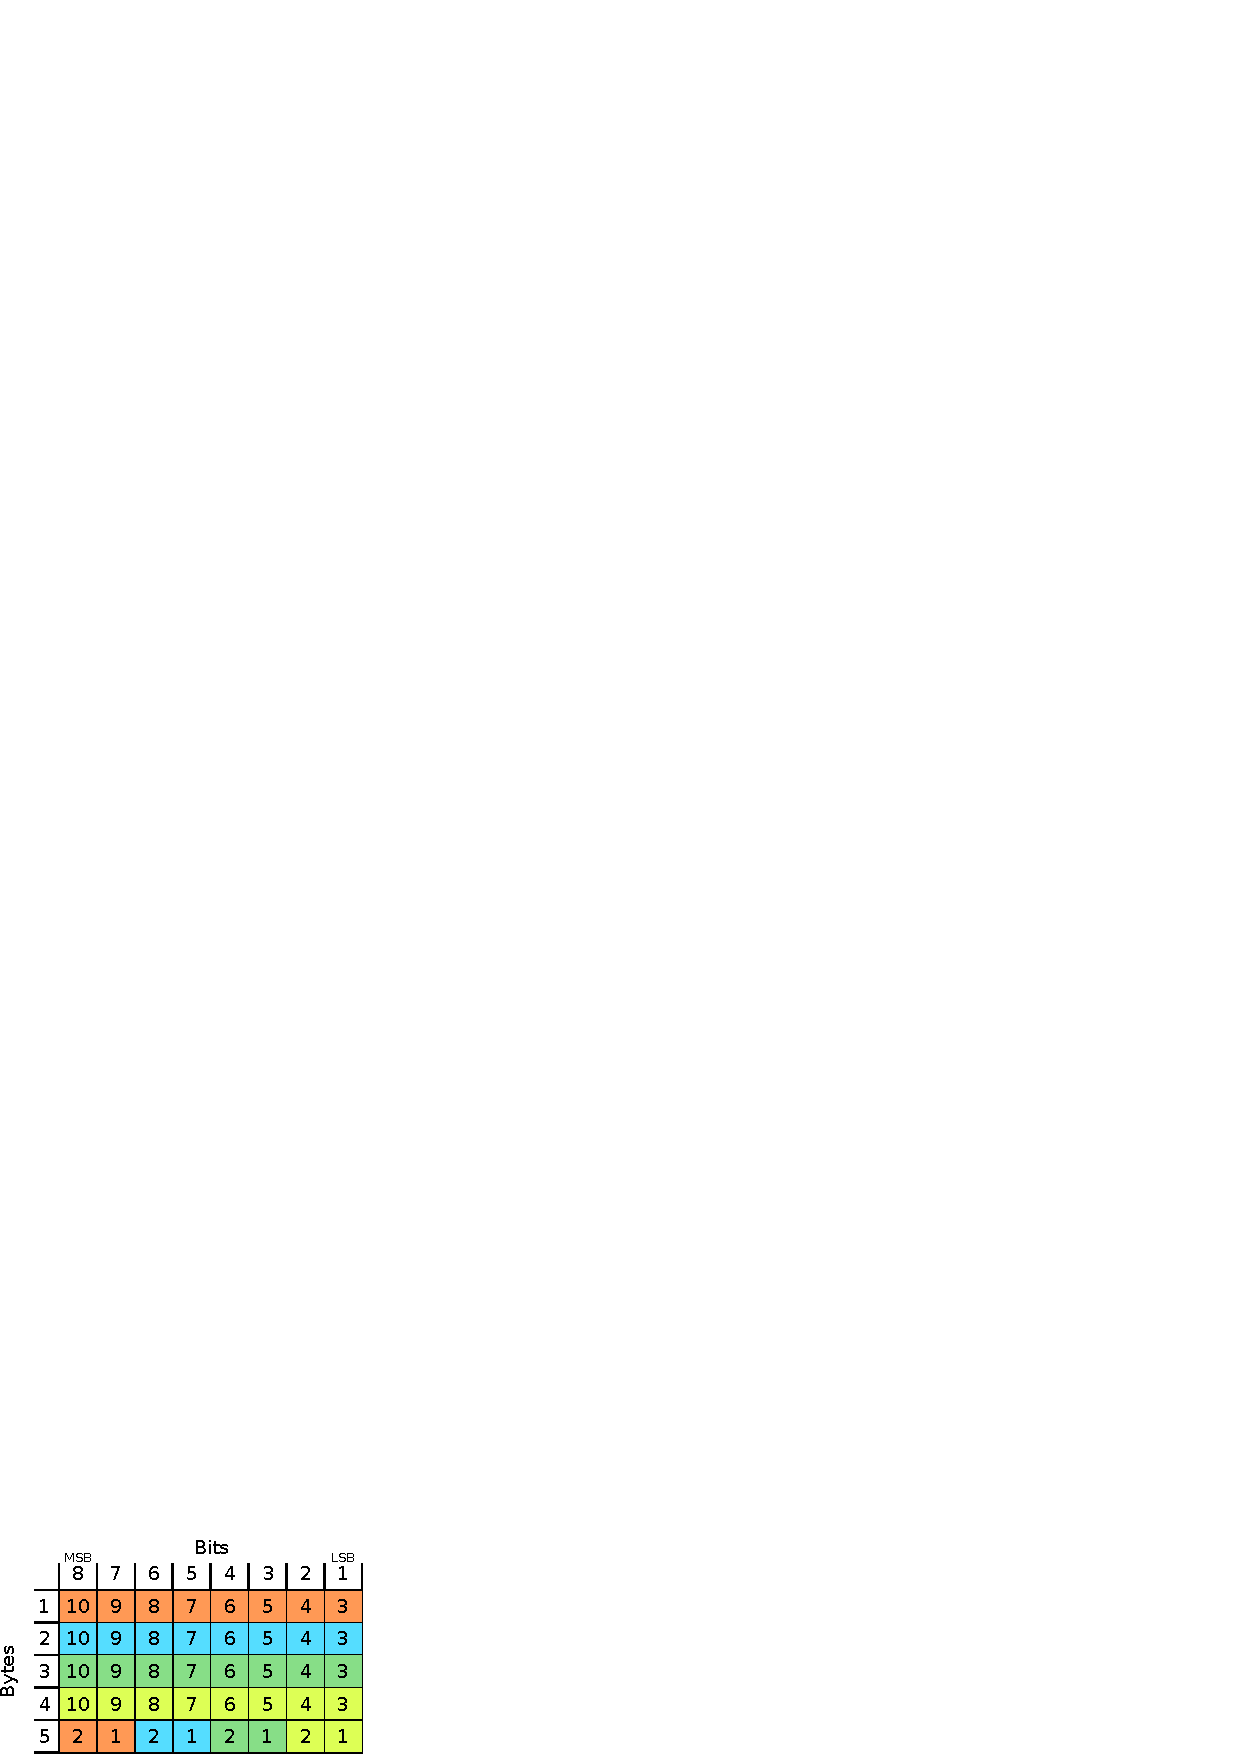
\includegraphics[width=0.8\textwidth]{figures/bayer_bytes.pdf}
    %    \label{fig:arreglo}
    %  \end{tikzfigure}
    %\end{minipage}
  }

  %%%%%%%%%%%%%%%%%%%%%%%%%%%%%
  \blocknode{Configuración Experimental}%
  {
    \subsection*{Emisor de rayos X}

      Se utilizó un emisor de rayos X de Cu para medir el espectro de este material.
      Con el mismo emisor, se intercalaron placas de Fe y Ca para determinar el espectro de estos materiales.
      En la Fig.\ref{fig:photo_xray} se muestra la configuración experimental utilizada.

      \begin{tikzfigure}[Configuración experimental utilizada para la detección de rayos X.
        El sensor se colocó dentro de un recipiente plástico para protogerla de la luz visible.]
        \includegraphics[width=0.75\textwidth]{figures/IMG_20180412_173110355_HDR}
        \label{fig:photo_xray}
      \end{tikzfigure}
  }

  %%%%%%%%%%%%%%%%%%%%%%%%%%%%

  \plainblock[3]{($(currenty)+(6,2)$)}{23}{Características de la \emph{Raspicam} V1.3\vspace{7mm}} %
  { 
    \begin{tabular}{ll}
      \textbf{Sensor:}                      & OmniVision OV5647                               \\
      \textbf{Precio:}                      & $\approx$ 23 dólares.                     \\
      \textbf{Cantidad de píxeles:}         & $2592$x$1944$                                   \\
      \textbf{Resolución:}                  & $5$ MP                                          \\
      \textbf{Tamaño de píxel:}             & \SI{1.4}{\micro\meter} x \SI{1.4}{\micro\meter} \\
      \textit{\textbf{Full Well Capacity:}} & 4300 electrones                                 \\
      \textbf{Profundidad de bits:}         & 10 bits por píxel                               \\
      \textbf{Tamaño de la imagen raw:}     & \SI{6.4}{\mega\byte}                           
    \end{tabular}
  }

  %%%%%%%%%%%%%%%%%%%%%%%%%%%%

  \blocknodew[($(currenty)-(12,0)$)]{12}{\Large Código Fuente}
  {
    \centering
    \includegraphics[width=\textwidth]{figures/QR_Code_GitHub.png}
    \href{https://github.com/DBFritz/ParticleDetections}{git.io/vhOLO}
  }
  

  %%%%%%%%%%%%% NEW COLUMN %%%%%%%%%%%%%%% 
  \startsecondcolumn 
  
  \blocknode{Resultados}%
  {
    \subsection*{Determinación del ruido de lectura}

      \begin{minipage}{0.5\linewidth}
        \coloredbox{colorthree!50!}{
          Se promediaron 30 fotografias para determinar el ruido de lectura por pixel.
          La imagen resultante se muestra en la Fig.~\ref{fig:background}

          Se realizó un histograma de los valores de los pixeles de una única imagen,
          para verificar la distribución y la dispersión del ruido.
          Los resultados obtenidos se muestran en la Fig.~\ref{fig:background}.

          Debido a la fuerte dependencia del ruido con la columna, se restó la media por columna
          a cada columna. El histograma resultante se muestra en la Fig.~\ref{fig:histogram_subs}
        }
      \end{minipage}
      \begin{minipage}{0.5\linewidth}
        \begin{tikzfigure}[Promedio de 30 imágenes sobre el fondo]
          \includegraphics[width=0.9\textwidth]{figures/background.jpg}
          \label{fig:background}
        \end{tikzfigure}
      \end{minipage}

      \begin{minipage}{.47\textwidth}
        \begin{tikzfigure}[Histograma obtenido para una imagen]
          \centering
          \includegraphics[width=\linewidth]{figures/background_histo.pdf}
          \label{fig:histogram}
        \end{tikzfigure}
      \end{minipage}%
      \begin{minipage}{.53\textwidth}
        \begin{tikzfigure}[Histograma obtenido para una imagen, con el promedio por columna restado]
          \centering
          \includegraphics[width=\linewidth]{figures/background_histo_subs.pdf}
          \label{fig:histogram_subs}
        \end{tikzfigure}
      \end{minipage}
    
    \vspace{10mm}
    \subsection*{Calibración y determinación de los picos $K_\alpha$ y $K_\beta$}

    \vspace{10mm}
    \subsection*{Detección de rayos cósmicos}
    \begin{minipage}{0.5\linewidth}
      \coloredbox{colorthree!50!}{
        Durante dos días de captura de video se analizaron los fotogramas en busca de eventos,
        en busca de detectar eventos producidos por rayos cósmicos secundarios.
        En total se encontraron 2, dichos eventos se muestran en la Fig.~\ref{fig:cosmic_rays}
      }
    \end{minipage}
    \begin{tikzfigure}[Histograma obtenido para una imagen, con el promedio por columna restado]
      \centering
      \includegraphics[width=\linewidth]{figures/doble_evento.png}
      \label{fig:cosmic_rays}
    \end{tikzfigure}

  }

  \blocknode{Conclusiones}
  {

  }

  \blocknodew[(0,43.5)]{67}
  {\hspace{28.5cm}\huge \texttt{Resumen} }
  {
      \large
      Los sensores CMOS constituyen una alternativa de bajo precio para la detección de interacciones de partículas.
      En este trabajo se implementó una librería para utilizar el sensor OmniVision OV5647
      de la cámara Raspicam V1.3, con una Raspberry Pi.
      Utilizando esta librería se observaron los picos de emisión de rayos X
      $K_{\alpha}$ y $K_{\beta}$ del Cu y los picos $K_{\alpha}$ del Fe y del Ca.
      La determinación de estos picos permitió hacer la correcta calibración de carga depositada en
      función del valor de los píxeles.
      Finalmente se utilizó la librería para la detección de interacciones con partículas secundarias
      producidas por rayos cósmicos con el sensor.
  }

\end{tikzpicture}

\end{document}




